\documentclass[12pt]{article}
\usepackage{mathtools,bm}
\usepackage{amsmath,amsfonts,amssymb}   %% AMS mathematics macros
\usepackage{graphicx}
\usepackage{fancyvrb}
\usepackage{color}
\usepackage{url}
\usepackage{hyperref}
\usepackage{authblk}
\usepackage{geometry}
\linespread{1.4}
 \geometry{
 a4paper,
 total={174mm,257mm},
 left=20mm,
 top=20mm,
 }
 \renewcommand{\floatpagefraction}{.8}
 \renewcommand\Affilfont{\fontsize{9}{10.8}\itshape}

\definecolor{lightblue}{rgb}{0.0,0.5,0.8}
\newcommand{\todo}[1]{\comment{{\color{lightblue}\par {[{\bf TO DO: } {\em #1}} ] \\    }}}
\newcommand{\addref}[1]{\comment{{\color{red}{\bf [REF #1]}}}}

 \title{Dynamic leaf sequencing via polynomial representations of leaf trajectories and dose rate}

 \author{Matthew Kelly, Koos van Amerongen, David Craft}
\affil[]{Department of Radiation Oncology, Massachusetts General Hospital, Harvard Medical School}
%% \date{February 13, 2016}

\begin{document}

\maketitle
\thispagestyle{empty}

%\begin{figure}[!htbp]
%\centering
%%trim option's parameter order: left bottom right top
%\includegraphics[trim=0 50 0 0,clip,width=17cm]{clonalTree}
%\caption{Clonal expansion of a cancer cell population. The population starts exponentially dividing with fitness $f_0$ at time 0.}
%\label{clonalTree}
%\end{figure}


\begin{abstract}
  We consider the problem of matching a given fluence map $f$ to a close approximation in limited time $T$ by the use
  of a multi-leaf collimator, i.e. the setting of IMRT and VMAT in radiation therapy. We use low order polynomial
  representations for leaf velocities and the dose rate as functions of time. The optimization then searches over the coefficients
  that define those polynomials, resulting in an optimization problem in a smaller dimension and one that is inherently smoother,
  thus focusing on global aspects of the solution and avoiding the noisy local minima that occur when solving the problem in the original
  space of leaf positions and dose rates vs time.
\end{abstract}


%~~~~~~~~~~~~~~~~~~~~~~~~~~~~~~~~~~~~~~~~~~~~~~~~~~~~~~~~~~~~~~~~~~~~~~~~~~~~~~~~~~~~~~~~~~~~~~~~~%
\section{Introduction}
The optimal dynamic delivery of a given fluence map remains a difficult,
largely unsolved problem, due to its inherent nonconvexity.
The nonconvexity of the fluence map matching problem leads to a large number of local minima.
Many methods simply ignore this crucial aspect of the problem,
and others use a multi-start procedure to find several local minima and return the best one found.
For a thorough introduction to the complexities of dynamic fluence map delivery
(which generally arises in the context of volumetric modulated arc therapy, VMAT),
see \cite{balvertcraft} and \cite{unkvmatreview}.

In this technical note, we investigate a regularization procedure which represents
leaf trajectories and dose rates as linear splines (piece-wise linear functions),
such that the optimization procedure naturally focuses on global aspects of the leaf trajectory/dose rate solution.


\subsection{Background}

\todo{ David  --  Would you be able to add any background that is appropriate for this paper,
at least from a fluence mapping perspective?  Let me know if I should add a short section about
trajectory optimization. Also, should background be its own section, or is a sub-section in the
Introduction acceptable?}
\KvAcomment{Did I forget to send my contribution to the introduction from quite a while ago as a pull request?} 

\subsection{Fluence Mapping as Continuous Optimization}
\label{sec:FluenceMappingAsContinuousOptimization}

Our goal is to compute the optimal leaf trajectories $x_L(t)$ and $x_R(t)$,
as well as the optimal dose rate $d(t)$ of the radiation source for $t\in[0,T]$.
For this initial study we will consider only a single leaf pair,
although our algorithm is structured such that it could be applied to an arbitrary number of leaf pairs.
We will assume that adjacent leaves are independent of each other,
neglecting the small coupling terms created by the tongue-and-groove mechanism on the real machine.

Let the position domain of the fluence profile be denoted by $X$.
We will assume that the target fluence at each floating point position $x\in X$, $f(x)$, is given.
Our goal is to find the leaf trajectories $x_L(t)$ and $x_R(t)$ and dose rate pattern $d(t)$
that minimize the squared integral error between the target fluence $f(x)$ and the delivered fluence $g(x)$:

\begin{equation}
\underset{d(t), \, x_L(t), \, x_R(t)}{\operatorname{argmin}}
\int_X \bigg(f(x)) - g(x)\bigg)^2 dx .
\label{eqn:fluenceMapOptimization}
\end{equation}

\vspace{6pt}

\todo{In practice, target fluence comes in discrete format, bixels. How to proceed on fixing this mismatch?
David, is there any chance FMO might give us continuous - or at least very precise - maps in the near future?}

The fluence delivered at each position, $g(x)$, is the time-integral of the dose rate for the times that position is exposed.
This time domain $\mathcal{T}(x)$ is the set of times when the position $x$ is not blocked by either of the leaves, i.e.,
$\mathcal{T}(x)$ is the set of all times $t$ such that $x_L(t) < x \leq x_R(t)$,
as illustrated by Figure \addref{exposure figure} .

\begin{equation}
g(x) = \int_{\mathcal{T}(x)} d(t) dt
\label{eqn:deliveredFluenceDose}
\end{equation}

For this work we will leave the initial and final leaf positions as decision variables in the optimization, 
but it is a trivial extension to enforce arbitrary initial and final leaf positions 
with a simple modification to the position limits at these points in the trajectory. 
This might be useful when combining a sequence of fluence maps as shown in \cite{balvertcraft}.

We will also assume that the available delivery time is given,
but this could easily be added as a decision variable at a later time.

% $x_L(0) = x_U(0)$ and
% $x_L(t) = x_U(T)$ where
% $t \in [0, T]$.


\subsection{Implementation as a Nested Optimization}

The optimization formulation presented in Section \S \ref{sec:FluenceMappingAsContinuousOptimization}
is a good mathematical description of our goal, but it is not obvious how to solve it.
In this paper we use a nested optimization approach,
solving the dose rate trajectory $d(t)$ in an outer optimization,
and then solving the optimal leaf trajectories $x_L(t)$ and $x_R(t)$ as an inner optimization,
given a candidate dose rate trajectory.

Partitioning the problem in this fashion makes physical sense: given a fixed dose rate trajectory,
the leaf trajectories are completely independent.
This decoupling allows us to focus on designing the inner and outer optimizations differently,
each specialized for the details of that optimization.

\todo{David - do we need an equation here?
    If so, I'm not sure of the best way to write the nested optimization.}

\KvAcomment{I'd formally formulate the inner and outer dose rate optimization problems, with objective and constraints and explaining which entities are variable and which operate as a parameter.}





%~~~~~~~~~~~~~~~~~~~~~~~~~~~~~~~~~~~~~~~~~~~~~~~~~~~~~~~~~~~~~~~~~~~~~~~~~~~~~~~~~~~~~~~~~~~~~~~~~%
\section{Method - Inner Optimization - Leaf Trajectories}


\subsection{Trajectory Representation}

The final goal of our optimization is to compute three trajectories:
radiation dose-rate $r(t)$, lower leaf position $z_L(t)$, and upper leaf position $z_U(t)$.
Each of these trajectories is represented by a piecewise linear spline,
with shared knot times $t_k \in \{t_0, t_1, \dots, t_N\}$, where $N$ is the number of knot points.
The value of the dose rate and leaf positions at knot time $t_k$ are given by
$r_k$, $x_{L,k}$, and $y_{U,k}$ respectively.

\begin{figure}
  \centering
  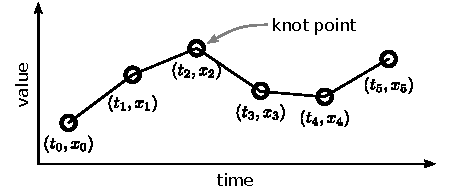
\includegraphics{fig/linearSpline.pdf}
  \caption{Linear Spline. We represent the dose-rate and leaf position trajectories as linear
           splines. A linear spline is fully defined by its value at the knot points. }
  \label{fig:linearSpline}
\end{figure}

\subsection{Trajectory Limits}

There are several constraints imposed on the dose-rate and leaf trajectories
by the physical limitations of the VMAT machine. Specifically, there is a maximum dose-rate,
constant limits on the leaf positions, and an upper limit on the leaf speed.
These limits are detailed below, where $\dot{z}(t) = \tfrac{d}{dt}z(t)$ gives the leaf velocity.
\begin{align}
  \text{dose-rate: }& \quad 0 \leq r(t) \leq r_\text{max}
      \label{eqn:FirstTrajectoryConstraint}\\
  \text{leaf position: }& \quad x_\text{min} \leq z_L(t) \leq z_U(t) \leq x_\text{max} \\
  \text{lower leaf velocity: }& \quad v_\text{min} \leq \dot{z}_L(t) \leq v_\text{max} \\
  \text{upper leaf velocity: }& \quad v_\text{min} \leq \dot{z}_U(t) \leq v_\text{max}
      \label{eqn:LastTrajectoryConstraint}
\end{align}

\subsection{Avoiding Local Minima}

One of the key issues with fluence mapping is that the
optimization tends to get stuck in local minima,
since there are a large number of leaf trajectories that deliver the same fluence to the target.
\addref{local minima in fluence mapping}

It is possible to help the optimization avoid local minima by smoothing the optimization problem.
This smoothing is useful because it means that the gradient estimates in the optimization change less
between each iteration in the optimization.

There is an obvious trade-off here: smoothing makes the optimization easier by fundamentally changing the problem statement,
thus we get an easy optimization that is inaccurate.
The solution here is to iteratively reduce the smoothing terms,
initially solving the optimization with heavy smoothing to avoid local minima,
and then using that solution to initialize another optimization with less smoothing.
See \S Section \ref{sec:modelingFluenceBlocking} for details.

This technique of iteratively reducing a smoothing term is widely used in trajectory optimization,
such is in \cite{Srinivasan2006}.


\subsection{Computing Delivered Fluence}

The fluence delivered at each position on the target is computed by integrating the
dose-rate function over the periods of time when the leaves are not blocking the target:

\begin{equation}
  f_D(x) = \int_{\mathcal{T}(x)} \! r(t) \,dt
  \quad \quad
  \mathcal{T}(x) = \forall t
  \quad
  \text{S.T.}
  \quad
  z_L(t) \leq x \leq z_U(t)
  \label{eqn:fluenceMapIntegral}
\end{equation}

There are two issues with computing this integral directory.
The first is that it requires either computing the inverse of the leaf trajectories,
which ultimately reduces to a non-linear root finding sub-problem.
When placed inside of an optimization, this will dramatically slow convergence.
The second issue is that the set $\mathcal{T}(x)$ does not smoothly vary with respect to the leaf trajectories.
It is possible to construct a set of leaf trajectories for which a small change in leaf position
switches $\mathcal{T}(x)$ from one to two simply connected sets.
Inside of an optimization, this would cause a change in the sparsity pattern of the gradient
(\textit{e.g.} $\tfrac{\partial f_D}{\partial z_L})$)
between successive iterations,
which leads to poor convergence and possibly a numerical instability.

Our solution is to rewrite the integral using a blocking function $k(t)$,
which has a value of one when the leaves are passing radiation and
zero when the leaves are blocking radiation, as described in \S\ref{sec:modelingFluenceBlocking}
This allows us to rewrite (\ref{eqn:fluenceMapIntegral}) using the constant bounds $[0, \mathcal{T}]$:

\begin{equation}
  f_D(x) = \int_0^T \! k(t, x) \cdot r(t) \, dt
  \label{eqn:fluenceDoseSimpleBounds}
\end{equation}

Now we have a standard scalar integral, where the integrand is smooth and the
bounds are constant, we can use any quadrature method to evaluate (\ref{eqn:fluenceDoseSimpleBounds}).
In this case we use the midpoint (rectangle) quadrature rule.

\subsection{Modeling Fluence Blocking}
\label{sec:modelingFluenceBlocking}

A simple way to define the fluence blocking function $k(t)$
would be to set it to one if $z_L(t) \leq x \leq z_U(t)$
is true, and zero otherwise.
This implementation would have a discontinuous gradient, which would cause problems in the optimization.
Instead, we use exponential smoothing to approximate the step function $s(x,\alpha)$,
where $\alpha$ is a small smoothing parameter.
A smaller smoothing parameter will provide a more accurate model,
while a larger smoothing parameter will lead to faster optimization.

\begin{equation}
  k(t, x) = \sqrt{s\big(x - z_L(t), \, \alpha\big) \; \cdot \; s\big(z_U(t) - z, \, \alpha\big)}
\end{equation}

\begin{equation}
  s(t, \alpha) = \frac{1}{1 + e^{-t/\alpha}}
\end{equation}

In practice it is useful to define the smoothing parameter $\alpha$ in terms of a smoothing distance ($\gamma$)
and the fraction change ($\Delta s$) in smoothing over this distance.

There is a physical interpretation of the smoothing distance $\gamma$ for the leaf-blocking model:
it is the distance, centered on the edge of the leaf, where the edge is blurred by the smoothing.

\begin{equation}
  \alpha = \frac{2}{\Delta s} \ln \left( \frac{1}{2} (1 - \gamma) \right)
\end{equation}


\subsection{Objective Function}

The objective function for the inner optimization (computing leaf trajectories)
is the integral of the error-squared between the target fluence $f_T(x)$ and the delivered fluence $f_D(x)$.
\begin{equation}
  J = \int_{x_\text{min}}^{x_\text{max}} \! \big( f_T(x) - f_D(x) \big)^2 \,dx
  \label{eqn:continuousFittingObjective}
\end{equation}

In practice we can only compute the fluence profile at a finite number of points.
We will break the domain $[x_\text{min}, x_\text{max}]$ into $N_\text{fit}$ equal-width segments,
and evaluate the fluence target and delivered fluence at the midpoint $x_k$ of each segment.
This is equivalent to approximating (\ref{eqn:continuousFittingObjective}) using rectangle (mid-point)
quadrature with $N_\text{fit}$ segments.

\begin{equation}
  J \approx \frac{x_\text{max} - x_\text{min}}{N_\text{fit}}\sum_{k = 1}^{N_\text{fit}} \! \big( f_T(x_k) - f_D(x_k) \big)^2
  \label{eqn:discreteFittingObjective}
\end{equation}

\subsection{Transcription to a Nonlinear Program}

The inner optimization loop computes the leaf trajectories $z_L(t)$ and $z_U(t)$
that minimize the objective function (\ref{eqn:FluenceFittingObjective})
and satisfy the constraints (\ref{eqn:FirstTrajectoryConstraint}--\ref{eqn:LastTrajectoryConstraint}).

The limits on leaf position can be implemented as a combination of
constant bounds and linear inequality constraints:

\begin{equation}
  x_\text{min} \leq x_{L, k}
  \quad \quad
  x_{U, k} \leq x_\text{max}
  \quad \quad
  x_{L, k} \leq x_{U, k}
  \quad \quad
  \forall k
\end{equation}

Since we represent these trajectories as piecewise linear,
it is natural to represent them by their values at the knot points $t_i$.
The position trajectory is piecewise linear,
and we can compute the velocity trajectory by taking the derivative of the spline.
The velocity between each pair of knot points will be constant and given by:

\begin{equation}
  \dot{z}_{L, k} = \frac{z_{L, k+1} - z_{L, k}}{h_k}
  \quad \quad
  \dot{z}_{U, k} = \frac{z_{U, k+1} - z_{U, k}}{h_k}
\end{equation}

The limits on velocity can thus be written as linear inequality constraints:

\begin{equation}
  v_\text{min} \leq \dot{z}_{L, k} \leq v_\text{max}
  \quad \quad
  v_\text{min} \leq \dot{z}_{U, k} \leq v_\text{max}
  \quad \quad \forall k
\end{equation}

\todo{Add a summary sentence about how to pack everything up into a NLP solver}


%~~~~~~~~~~~~~~~~~~~~~~~~~~~~~~~~~~~~~~~~~~~~~~~~~~~~~~~~~~~~~~~~~~~~~~~~~~~~~~~~~~~~~~~~~~~~~~~~~%


\section{Method - Outer Optimization - Dose Rate Trajectories}

\todo{Write this section.}

Proposed Method (yet to be tested):  Start by running CMAES witha wide search and heavy smoothing
parameters. Optimize over the smoothed objective at the low level, but then spend the extra CPU
time to benchmark the actual value of each solution. Once this optimization converges, then
run a second round of CMAES using iterative smoothing refinement.

\subsection{Objective Function:}

Best leaf trajectories!

\todo{Finish writing}

\subsection{Optimization:}

CMAES
\todo{Finish writing}


\section{Methods - template}

[MATT this is copy and pasted from the original ``chebyopt.pdf'' that I sent you. Probably all will need to be revised, but leaving it in case some is salvagable/usable.]

We consider a single row version of the problem. Extension to the full fluence map should be possible, but it makes sense
to first develop the method and see how it works for a single row. Let $f(x)$ be the desired fluence map to deliver, where
$x$ is the position across the fluence row, $x \in [-1,1]$. We choose this as the domain because that is the
domain that the Chebyshev polynomials are written for. Across that domain the Chebyshev polynomials range from $-1$ to $1$.
We assume we have $T=1$ time unit to reproduce the fluence map $f$ by sliding leaves across the field from left to right.
Let $v_L(t)$ be the velocity of the left leaf at time $t$ and $v_R(t)$ the right leaf velocity. We assume we fix the starting positions
of both leaves. We may end up assuming we fix the ending positions too. This is not ideal, in fact we would like to optimize over
starting and ending leaf positions as well, but to make things more concrete, for now starting positions are assumed fixed and given.

Let $x_L(t)$ be position of the left leaf at time $t$. We have
\begin{equation}
  x_L(t) = x_L(0) + \int_{\tau=0}^t v_L(\tau) d\tau.
\end{equation}
\noindent (ditto for right leaf). Let $T_L(x)$ be the inverse of this function
(if we assume/enforce that velocity is always $>0$ then this inverse exists). Thus
$T_L(x)$ is the time that the left leaf crosses the position $x$. The fluence delivered to position
$x$, which we call $g(x)$ is the integration of the dose rate over the interval for which the position $x$ is not covered by either leaves,
see Figure \todo{sketch}.

%\begin{figure}[!htbp]
%\centering
%%trim option's parameter order: left bottom right top
%\includegraphics[trim=0 0 0 0,clip,width=12cm]{sketchCheby.pdf}
%\caption{Sketch of two leaf trajectories and the integration range (dotted line) for computing $g(x)$.}
%\label{sketch}
%\end{figure}

\begin{equation}
  g(x) = \int_{t = T_R(x)}^{T_L(x)} d(t) dt
\end{equation}
\noindent where d(t) is the dose rate at time $t$.

The optimization problem is to find the velocities and the dose rate over time to get $g$ as close to $f$ as possible:

\begin{equation}
\mathrm{min} \int_{x=-1}^1 \left ( g(x) - f(x) \right )^2 dx
\end{equation}

ENTER THE CHEBYSHEVS: We represent the velocities $v$ as weighted sums of Chebyshev polynomials of the first kind.
Here are the first four, for ease of reference:
$$
T_0(t) = 1
$$
$$
T_1(t) = t
$$
$$
T_2(t) = 2t^2 -1
$$
$$
T_3(t) = 4t^3 - 3t
$$

%$$[ 1, x, 2*x^2 - 1, 4*x^3 - 3*x, 8*x^4 - 8*x^2 + 1]

So, for example, the left leaf velocity is given by
$$
v_L(t) = \sum_{i=0}^3 c^L_i T_i(t).
$$
\noindent and we can do the same for the right leaf velocity and the dose rate as a function of time.
The optimization problem them becomes a search for the coefficients $c^L_i$, $c^R_i$, and $c^d_i$ that minimize the objective in Equation \ref{opt}.

\section{Results}

TODO:  results

\section{Discussion and conclusions}

\bibliographystyle{unsrt}
\bibliography{all}

\end{document}
